% 2007 年江苏卷第 18 题：棱长为 3 的正方体 ABCD-A1B1C1D1 及截面 EBFD1。
%   E 在 AA1 上（AE=1），F 在 CC1 上（FC1=1，CF=2）；
%   G 在 BC 上（BG=2/3），M 在 BB1 上，GM⊥BF 于 H。
% 来源 PDF：gaokaomath-src/普通高考/2007/2007江苏.pdf
% SHA-256：7b4d43a19a62295e52243f5c84485ce02fc6d00e98197482a09075d1c0e60bc0
% 原页：2007江苏.pdf 第 1 页（A3 三栏）第 3 栏，书页码 383。
% 重绘依据：按原页正方体斜投影、截面与 G/M/H 的位置重绘，尺寸比例按棱长 3。
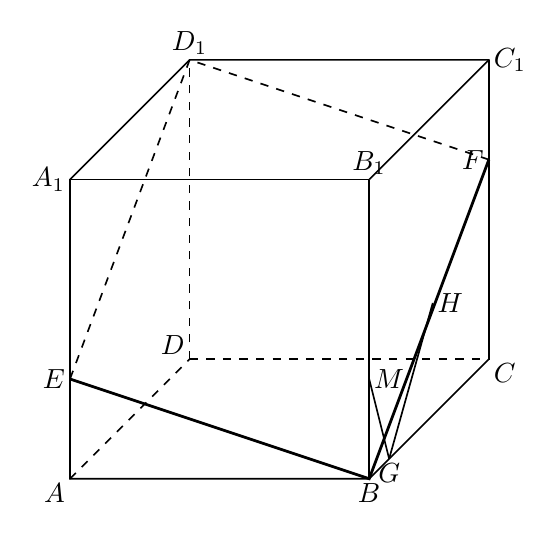
\begin{tikzpicture}[scale=0.95, semithick,
  every node/.style={inner sep=1.5pt}]

  % 正方体顶点（斜二测投影）
  \coordinate (A)  at (0,0);
  \coordinate (B)  at (4,0);
  \coordinate (C)  at (5.6,1.6);
  \coordinate (D)  at (1.6,1.6);
  \coordinate (A1) at (0,4);
  \coordinate (B1) at (4,4);
  \coordinate (C1) at (5.6,5.6);
  \coordinate (D1) at (1.6,5.6);

  % 被遮挡的棱
  \draw[dashed] (A) -- (D);
  \draw[dashed] (D) -- (C);
  \draw[dashed] (D) -- (D1);

  % 可见的棱
  \draw (A) -- (B) -- (C) -- (C1) -- (D1) -- (A1) -- cycle;
  \draw (A) -- (A1);
  \draw (B) -- (B1);
  \draw (C) -- (C1);
  \draw (B1) -- (C1);
  \draw (A1) -- (B1);

  % E、F、G、M
  \coordinate (E) at (0,1.3333);
  \coordinate (F) at (5.6,4.2667);
  \coordinate (G) at (4.2667,0.2667);
  \coordinate (M) at (4,1.3333);

  % 截面 E-B-F-D1-E
  \draw[line width=1pt] (E) -- (B) -- (F);
  \draw[dashed] (F) -- (D1);
  \draw[dashed] (D1) -- (E);

  % GM 与垂足 H（H 在 BF 上，取近似位置）
  \coordinate (H) at (4.85,2.35);
  \draw (G) -- (M);
  \draw (G) -- (H);

  % 标注
  \node[below left] at (A) {$A$};
  \node[below] at (B) {$B$};
  \node[below right] at (C) {$C$};
  \node[above left] at (D) {$D$};
  \node[left] at (A1) {$A_1$};
  \node[above] at (B1) {$B_1$};
  \node[right] at (C1) {$C_1$};
  \node[above] at (D1) {$D_1$};
  \node[left] at (E) {$E$};
  \node[left] at (F) {$F$};
  \node[below] at (G) {$G$};
  \node[right] at (M) {$M$};
  \node[right] at (H) {$H$};
\end{tikzpicture}
